% Prezentacja - etap 5 (18.XI). Skrypt wystąpienia: ../SKRYPT.md.
% Kompilacja: ../../.tools/bin/tectonic prezentacja.tex
\documentclass[aspectratio=169,11pt]{beamer}

\usetheme[progressbar=frametitle,numbering=fraction]{metropolis}
\usepackage[polish]{babel}
\usepackage{booktabs}
\usepackage{tabularx}
\usepackage{listings}
\usepackage{xcolor}
\usepackage{amssymb}
\usepackage{tikz}
\usetikzlibrary{arrows.meta,positioning}

\graphicspath{{../diagramy/}{img/}}
\newcolumntype{L}{>{\raggedright\arraybackslash}X}

\definecolor{ok}{HTML}{11804B}
\definecolor{bad}{HTML}{C0392B}
\definecolor{warn}{HTML}{A15C00}
\definecolor{acc}{HTML}{1F5EFF}
\newcommand{\good}[1]{\textcolor{ok}{#1}}
\newcommand{\bad}[1]{\textcolor{bad}{#1}}

\lstset{
  basicstyle=\ttfamily\footnotesize,
  keywordstyle=\color{acc}\bfseries,
  commentstyle=\color{gray},
  language=Python,
  columns=fullflexible,
  keepspaces=true,
  frame=none,
  backgroundcolor=\color{black!4},
  xleftmargin=4pt, framexleftmargin=4pt,
  extendedchars=true,
  literate={ą}{{\k{a}}}1 {ę}{{\k{e}}}1 {ó}{{\'o}}1 {ś}{{\'s}}1 {ł}{{\l}}1 {ż}{{\.z}}1 {ź}{{\'z}}1 {ć}{{\'c}}1 {ń}{{\'n}}1,
}

% pełnoekranowy diagram
\newcommand{\fullimage}[2][0.98]{%
  \begin{frame}[plain]
    \begin{tikzpicture}[remember picture, overlay]
      \node at (current page.center) {\includegraphics[width=0.99\paperwidth,height=#1\paperheight,keepaspectratio]{#2}};
    \end{tikzpicture}
  \end{frame}}

\title{System zapisów na zajęcia -- USOSv2}
\subtitle{Etap 5: projekt końcowy -- zapisy według preferencji, brak kolizji}
\author{Kamil Kręcigłowa \and Bartosz Królik \and Krzysztof Krówka}
\institute{Inżynieria Oprogramowania, zima 2026/2027}
\date{18 listopada 2026}

\begin{document}

\maketitle

% 1 ------------------------------------------------------------------ 0:50
\begin{frame}{Zadanie etapu 5 i punkt wyjścia}
  \small
  \begin{columns}[T]
    \begin{column}{0.5\textwidth}
      \textbf{Nowa funkcjonalność}\\[2pt]
      \footnotesize zapisy nie ,,kto pierwszy'', lecz według \textbf{preferencji}: student nadaje przedmiotom \textbf{wagi}, system \textbf{optymalizuje} przydział; wagi można \textbf{zmieniać w trakcie zapisów}.\\[8pt]
      \small\textbf{Testy}\\[2pt]
      \footnotesize brak kolizji w planie studenta przy zapisie, \textbf{zmianie harmonogramu w trakcie zapisów} i \textbf{przydziale z kolejki}.
    \end{column}
    \begin{column}{0.46\textwidth}
      \textbf{Punkt wyjścia}\\[2pt]
      \footnotesize z otrzymanego projektu mieliśmy tylko slajdy (Celery, Redis, kolejka FIFO) -- bez kodu.\\[4pt]
      Rozszerzenie zbudowaliśmy na \textbf{naszym działającym systemie} z etapów 1--3: FastAPI, PostgreSQL, worker, React.\\[4pt]
      \good{Wszystko poniżej jest zaimplementowane i przetestowane}: \textbf{96 testów}, w tym 61 nowych.
    \end{column}
  \end{columns}
\end{frame}

% 2 ------------------------------------------------------------------ 1:45
\begin{frame}{Tura preferencyjna -- jak to działa}
  \begin{columns}[T]
    \begin{column}{0.52\textwidth}
      \scriptsize
      \begin{enumerate}
        \item Dziekanat tworzy turę w trybie \texttt{PREFERENCES} z \textbf{pulą 100 pkt}.
        \item Student rozdziela punkty między przedmioty i układa akceptowane grupy w kolejności; \textbf{zmienia to dowolnie często} do zamknięcia tury.
        \item Co 5 min worker liczy \textbf{symulację}: student widzi przewidywany przydział i powody odmów, więc może zmienić wagi.
        \item Po zamknięciu worker \textbf{raz} wykonuje przydział końcowy, a wynik trafia do planów.
      \end{enumerate}
      \vspace{2pt}
      \textbf{Wspólna pula} wymusza wybór, co jest najcenniejsze, i daje wszystkim równe szanse. Remis rozstrzyga losowanie z \textbf{zapisanym ziarnem}, więc każdy wynik da się odtworzyć.
    \end{column}
    \begin{column}{0.46\textwidth}
      \centering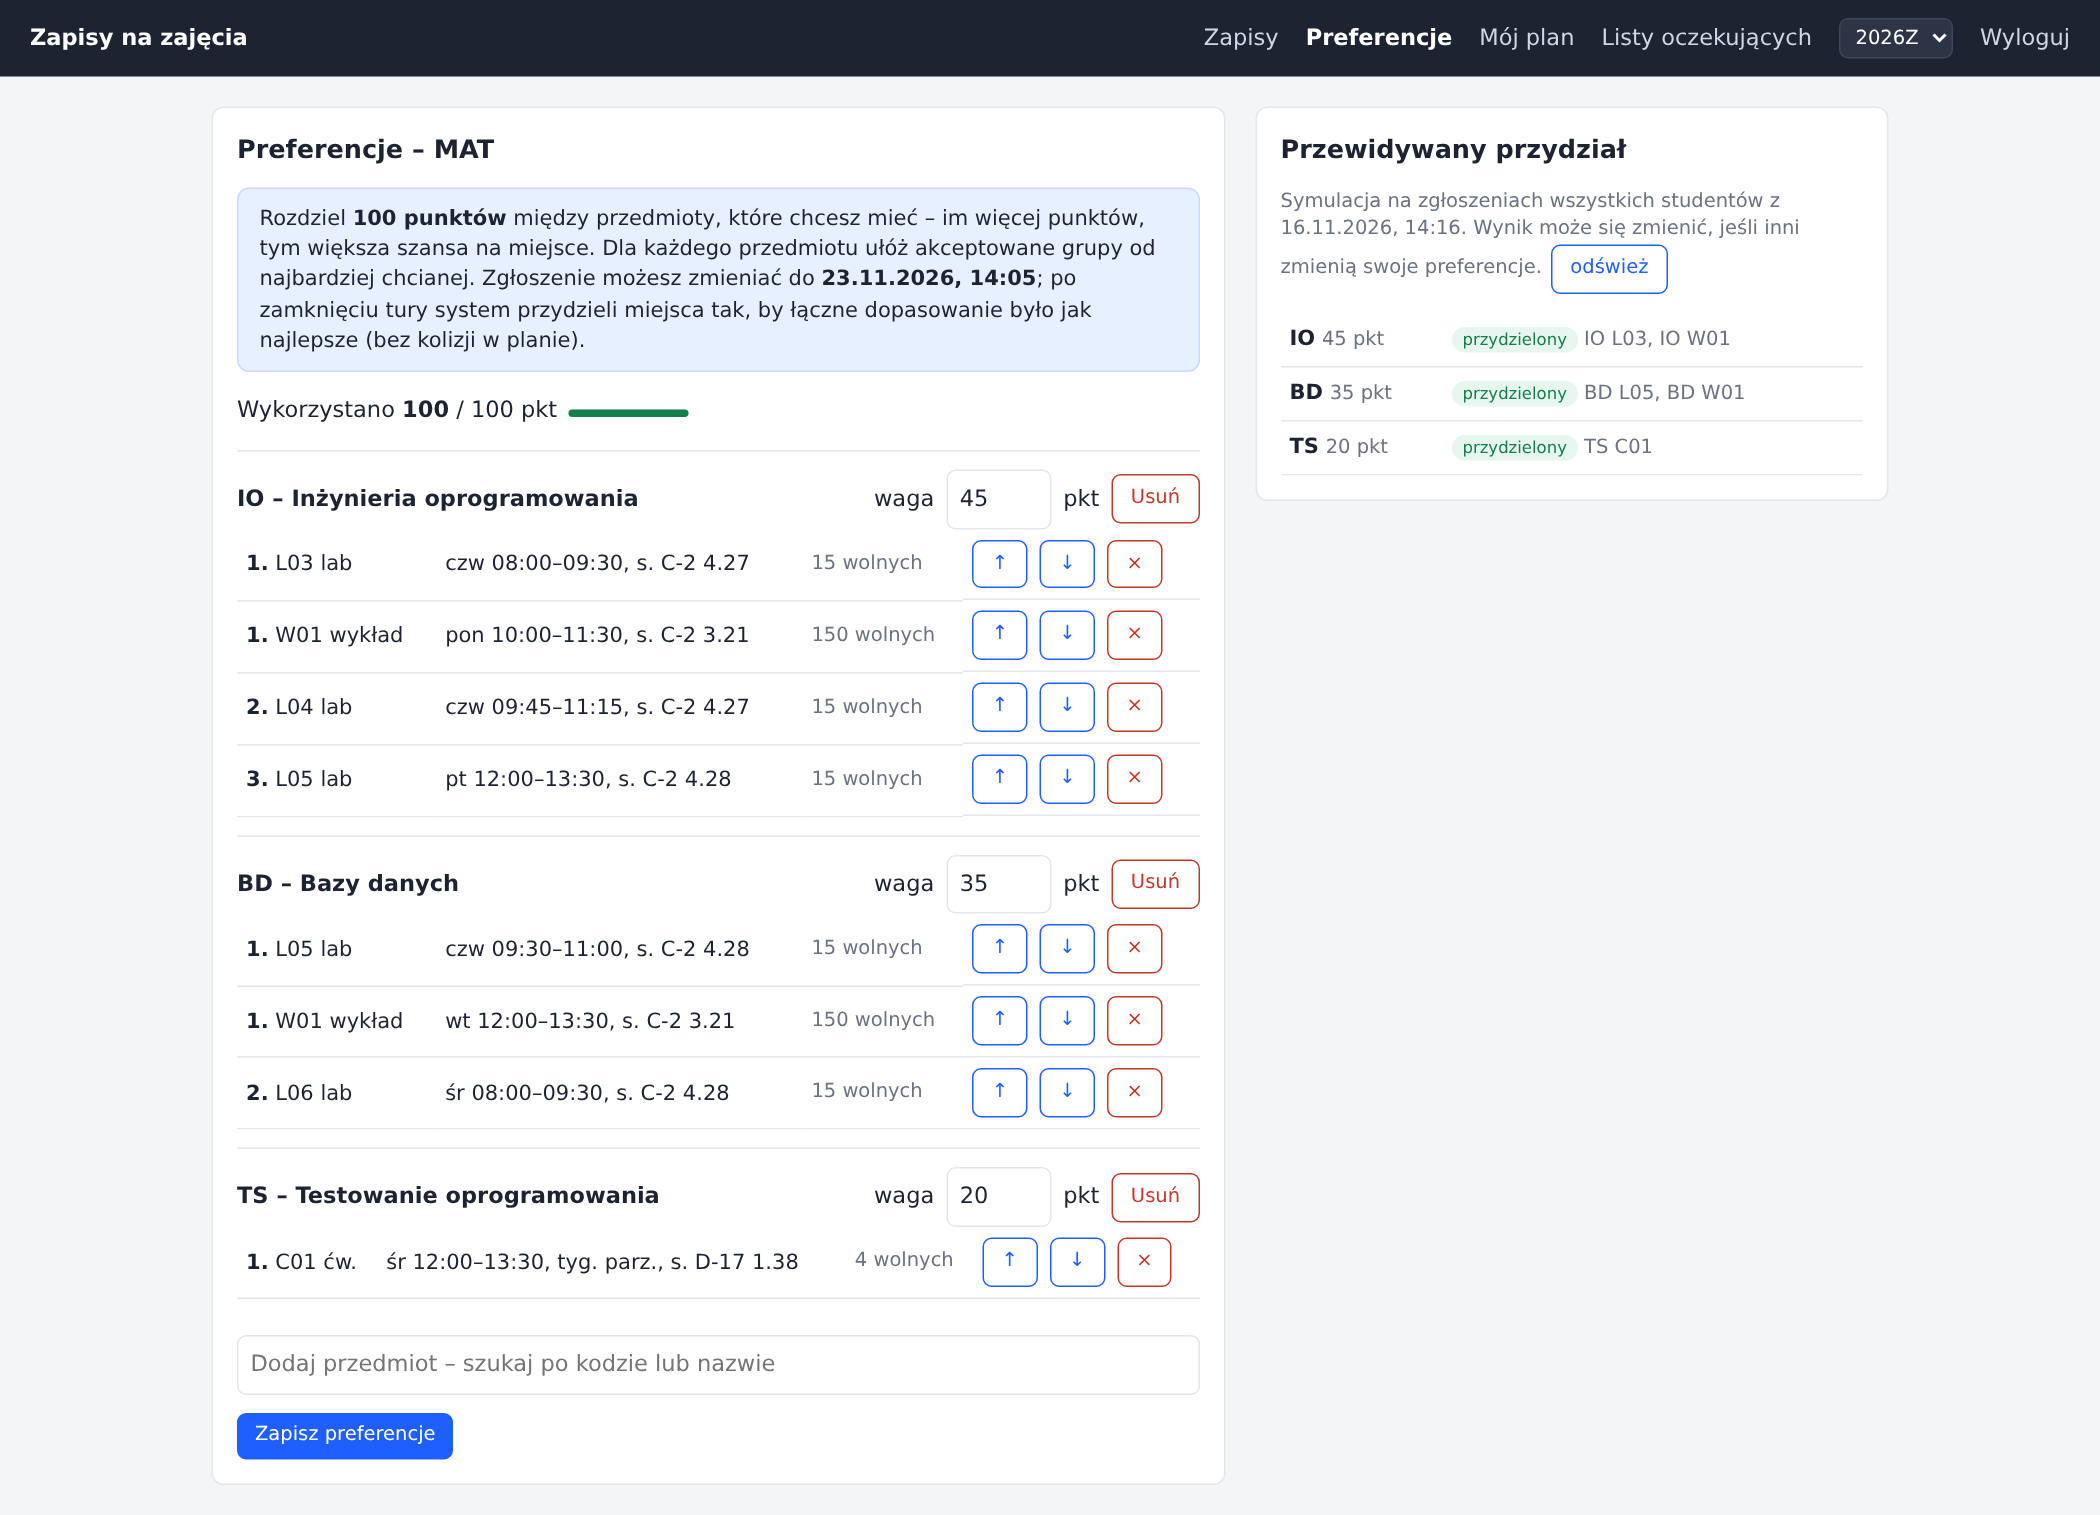
\includegraphics[width=\textwidth,height=0.8\textheight,keepaspectratio]{ui_preferencje.png}
    \end{column}
  \end{columns}
\end{frame}

% 3 ------------------------------------------------------------------ 2:20
\fullimage{przypadki_uzycia_preferencje.png}

% 4 ------------------------------------------------------------------ 3:15
\begin{frame}{Optymalizator przydziału}
  \scriptsize
  \textbf{Cel:} $\max \sum u$, \quad $u = \text{waga} \cdot \text{średnia}\big(\max(0.5,\; 1 - 0.1\,(\text{ranga}-1))\big)$ \quad -- waga decyduje \emph{czy}, ranga -- \emph{którą grupę}.\\
  \textbf{Ograniczenia} jak przy zapisie: limity miejsc, \textbf{brak kolizji}, wymagania wstępne, jedna grupa danego typu, wykład + lab: wszystko albo nic.\\[3pt]
  Kolizje czynią problem NP-trudnym, więc stosujemy heurystykę o \textbf{zmierzonej} jakości:
  \begin{enumerate}
    \item wykonalne kombinacje grup każdego zgłoszenia (inne odpadają z powodem),
    \item zachłannie: malejąco po wadze, remis -- los z ziarnem,
    \item poprawa lokalna: przeniesienie kogoś do jego innej grupy (łańcuch do 2), zwolnienie tańszego przydziału, wycofanie ruchu, który nie zwiększa sumy.
  \end{enumerate}
  \begin{tabularx}{\textwidth}{@{}L>{\raggedleft}p{2.6cm}>{\raggedleft}p{2.2cm}>{\raggedleft\arraybackslash}p{2.8cm}@{}}
    \toprule
    \textbf{1000 losowych instancji vs przegląd zupełny} & \textbf{średnio optimum} & \textbf{najgorszy} & \textbf{dokładnie optimum} \\
    \midrule
    sam algorytm zachłanny & 98,1\,\% & \bad{55\,\%} & 83,9\,\% \\
    zachłanny + poprawa lokalna & \good{99,8\,\%} & 80\,\% & \good{97,1\,\%} \\
    \bottomrule
  \end{tabularx}\\[3pt]
  Skala kierunku: 1000 studentów $\times$ 6 przedmiotów -- ok.\ \textbf{7\,s}. Przed zapisem \texttt{verify()} niezależnie sprawdza wynik.
\end{frame}

% 5 ------------------------------------------------------------------ 4:00
\fullimage[0.92]{sekwencja_przydzial_skrot.png}

% 6 ------------------------------------------------------------------ 4:35
\begin{frame}{Model danych -- rozszerzenie (migracja 0002)}
  \begin{columns}[c]
    \begin{column}{0.62\textwidth}
      \centering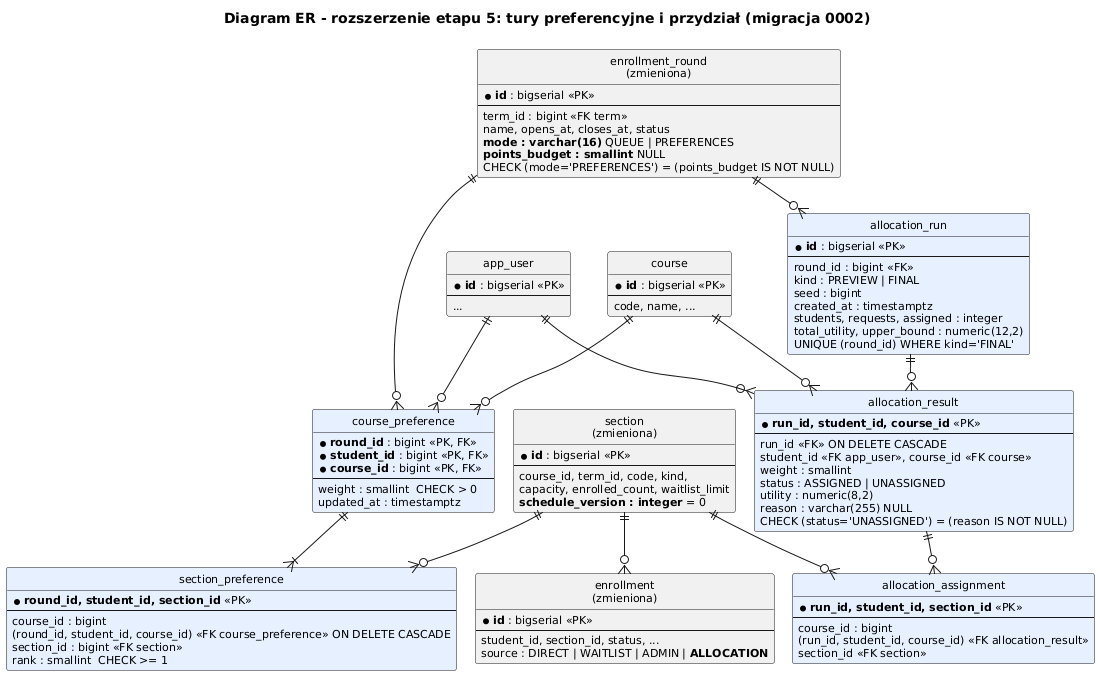
\includegraphics[width=\textwidth,height=0.85\textheight,keepaspectratio]{er_preferencje.png}
    \end{column}
    \begin{column}{0.36\textwidth}
      \scriptsize
      \begin{itemize}
        \item \texttt{course\_preference}: waga; suma $\le$ pula -- pod blokadą studenta
        \item \texttt{section\_preference}: ranga; FK złożony do zgłoszenia
        \item \texttt{allocation\_run}: PREVIEW / FINAL, ziarno, statystyki; \textbf{UNIQUE: jeden FINAL na turę}
        \item \texttt{allocation\_result}: każda odmowa ma powód (\texttt{CHECK})
        \item \texttt{section.schedule\_version}, \texttt{enrollment.source = ALLOCATION}
      \end{itemize}
    \end{column}
  \end{columns}
\end{frame}

% 7 ------------------------------------------------------------------ 5:20
\begin{frame}{Testy wykryły dwie luki -- zmiana terminu w trakcie tury}
  \footnotesize
  W etapie 3 sami wpisaliśmy je jako ,,znane ograniczenia'':
  \begin{enumerate}
    \item dziekanat przenosił termin grupy \bad{bez sprawdzania planów zapisanych studentów},
    \item zapis brał terminy z cache procesu (do 10\,s) -- \bad{inny proces API mógł przepuścić kolizję}.
  \end{enumerate}
  \textbf{Poprawki (UC32):}
  \begin{itemize}
    \item zmiana terminu: blokady sala/prowadzący $\rightarrow$ grupa $\rightarrow$ zapisani studenci (\texttt{NOWAIT}); kolizja u kogokolwiek $\Rightarrow$ \texttt{409 STUDENT\_CONFLICT} z listą indeksów,
    \item \texttt{section.schedule\_version}: zapis i awans z kolejki porównują wersję \textbf{pod blokadą grupy} -- różnica $\Rightarrow$ świeże terminy i ponowne sprawdzenie,
    \item oczekujący dostają powiadomienie; przy awansie kolizja $\Rightarrow$ \texttt{SKIPPED} z powodem,
    \item audyt niezmienników: \textbf{kolizja w planie} -- niezależna implementacja w SQL (wyrocznia testów, monitoring co minutę).
  \end{itemize}
\end{frame}

% 8 ------------------------------------------------------------------ 5:55
\fullimage[0.92]{sekwencja_zmiana_terminu_skrot.png}

% 9 ------------------------------------------------------------------ 6:45
\begin{frame}[fragile]{Scenariusze testowe: przygotowanie -- test -- weryfikacja}
  \begin{columns}[T]
    \begin{column}{0.5\textwidth}
\begin{lstlisting}[basicstyle=\ttfamily\scriptsize]
# K14: stary termin w cache innego procesu
# 1. przygotowanie
a = section(AAA, pon 10:00)
b = section(BBB, wt 10:00)
enroll(st, a)
load_target(b)        # cache: wtorek
update_meeting(b, pon 10:30)
                      # cache nie czyszczony
# 2. test
enroll(st, b)
# 3. weryfikacja
-> 409 CONFLICT
plan(st) == {AAA L01}
audit.violations() == []
\end{lstlisting}
    \end{column}
    \begin{column}{0.48\textwidth}
      \scriptsize
      \begin{tabular}{@{}p{4.3cm}r@{}}
        \toprule
        \textbf{grupa} & \textbf{testów} \\
        \midrule
        K -- kolizje (zapis, listy, awans, zmiana terminu, wyścigi) & 23 \\
        P -- tura preferencyjna (baza + API) & 17 \\
        A -- optymalizator (jakość, skala) & 21 \\
        etap 3 & 35 \\
        \midrule
        \textbf{razem} -- \good{wszystkie przechodzą} & \textbf{96} \\
        \bottomrule
      \end{tabular}\\[6pt]
      Wyścigi powtarzane 5--12 razy. Kontrola mutacyjna: wyłączenie wersji harmonogramu $\Rightarrow$ \bad{K13--K16 padają}.\\[3pt]
      Wszystkie scenariusze z wywołaniami: \texttt{etap5/TESTY.md}.
    \end{column}
  \end{columns}
\end{frame}

% 10 ----------------------------------------------------------------- 7:00
\begin{frame}[standout]
  Dziękujemy -- pytania?\\[8pt]
  \normalsize dokumentacja: \texttt{etap5/README.md}, \texttt{etap5/TESTY.md}\\
  dalej: slajdy zapasowe
\end{frame}

\appendix
\section{Slajdy zapasowe}

\fullimage{architektura.png}
\fullimage{aktywnosc_przydzial.png}
\fullimage{sekwencja_przydzial.png}
\fullimage{sekwencja_zmiana_terminu.png}
\fullimage[0.94]{sekwencja_preferencje.png}
\fullimage{klasy_przydzial.png}
\fullimage{klasy_serwisy.png}
\fullimage{klasy_domena.png}
\fullimage{klasy_infrastruktura.png}
\fullimage{przypadki_uzycia_student.png}
\fullimage{przypadki_uzycia_administracja.png}
\fullimage{er.pdf}
\fullimage[0.94]{sekwencja_zapis.png}
\fullimage[0.94]{sekwencja_wypis_awans.png}

\begin{frame}{Panel dziekanatu: tury i raport przydziału}
  \centering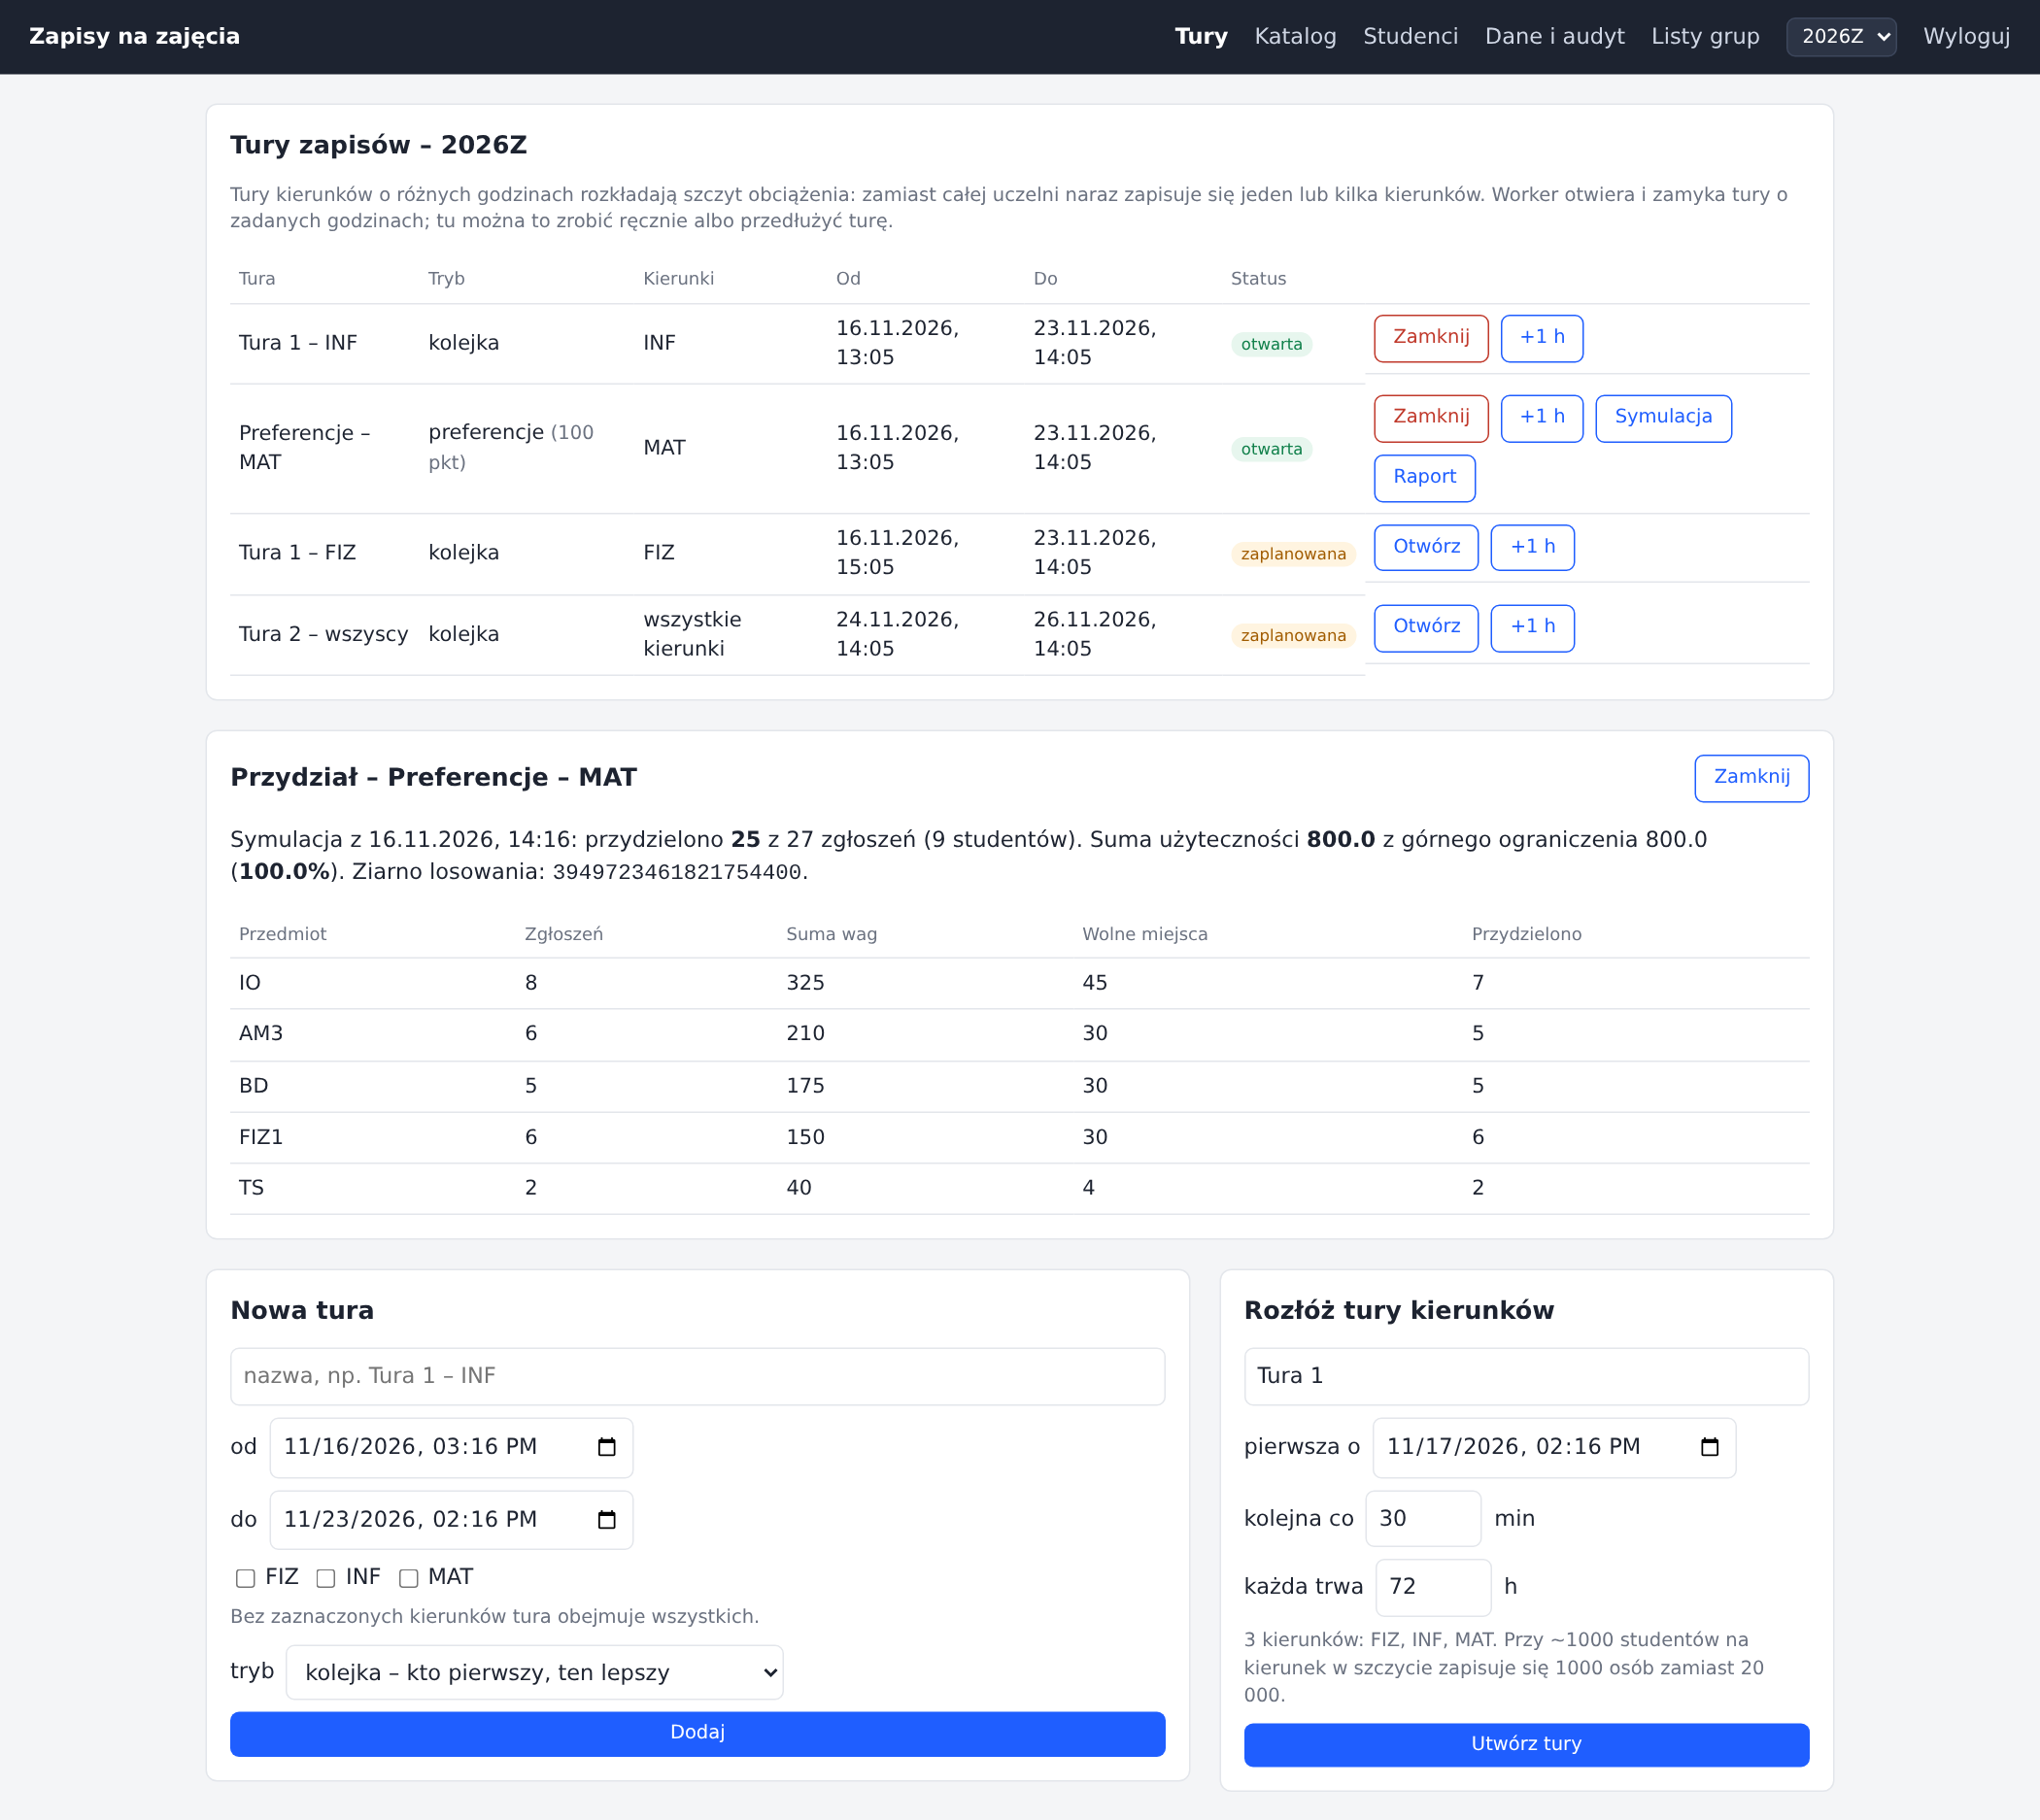
\includegraphics[width=\textwidth,height=0.82\textheight,keepaspectratio]{ui_tury.png}
\end{frame}

\begin{frame}{Co może pójść nie tak -- i co wtedy}
  \scriptsize
  \begin{tabularx}{\textwidth}{@{}>{\raggedright}p{5.2cm}L@{}}
    \toprule
    \textbf{Sytuacja} & \textbf{Reakcja} \\
    \midrule
    budżet przekroczony, obca grupa, przedmiot 2$\times$ & 409 z kodem; poprzednie zgłoszenie bez zmian (jedna transakcja) \\
    tura zamyka się w chwili zapisu preferencji & \texttt{FOR SHARE} na turze: zgłoszenie wchodzi do przydziału albo \texttt{ROUND\_CLOSED} (test P5) \\
    brak zaliczenia / kolizja z planem w zgłoszeniu & przyjęte z ostrzeżeniem; przydział sprawdzi ponownie \\
    dwie instancje workera, worker + dziekanat & blokada tury + \texttt{UNIQUE} FINAL $\Rightarrow$ \texttt{ALREADY\_ALLOCATED} \\
    awaria workera w trakcie przydziału & ROLLBACK, tura dalej ,,bez FINAL'' -- przydział od nowa \\
    miejsca zajęte / termin zmieniony po zgłoszeniu & przydział pod blokadami na stanie z chwili wykonania (P9, P12) \\
    błąd w optymalizatorze & \texttt{verify()} + \texttt{CHECK} w bazie $\Rightarrow$ nic nie zapisano \\
    zmiana terminu koliduje u zapisanego & \texttt{STUDENT\_CONFLICT} z listą indeksów \\
    student zapisuje się w trakcie zmiany terminu & \texttt{NOWAIT} + ponowienie albo wersja harmonogramu (K16) \\
    \bottomrule
  \end{tabularx}
\end{frame}

\end{document}
